\chapter{Performance results} % Main chapter title

\label{Chapter4} 

\section{Largest contentful paint}

\begin{figure}[h!]
	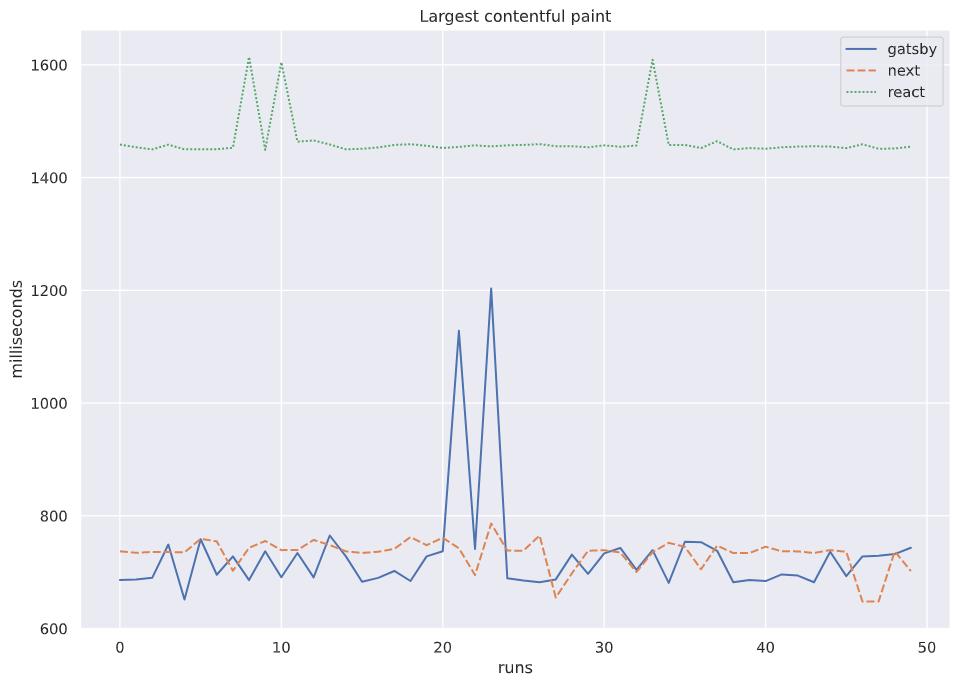
\includegraphics[scale=0.4]{largest_contentful_paint}
	\caption{Results of performance benchmark for largest contentful paint}
	\label{fig:largest_contentful_paint}
\end{figure}

In the figure, it is clear that LCP for a traditional React application is far greater than that of static site generators.

This makes sense: a traditional React application will perform many computational steps during runtime to render the DOM.
Static site generators will perform these computations during the build step.

\section{Total blocking time}


\begin{figure}[h!]
	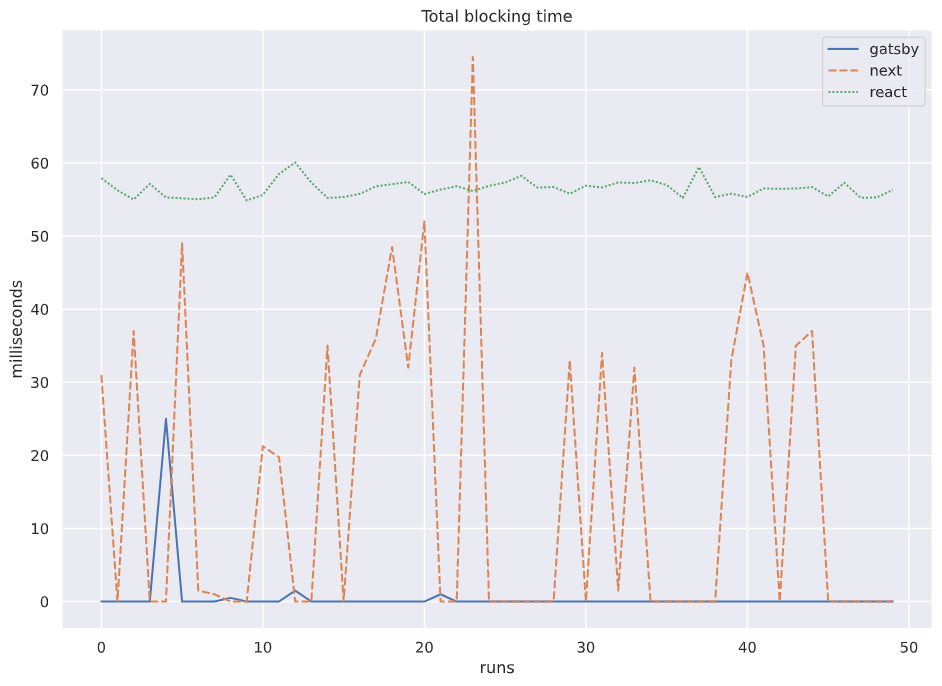
\includegraphics[scale=0.4]{total_blocking_time}
	\caption{Results of performance benchmark for total blocking time}
	\label{fig:total_blocking_time}
\end{figure}

Similar results from the previous figure can be observed. 
The traditional React application scores much less favorably than the static site generators.
Interestingly, the results for Next seem to spike a lot.